\chapter{Narrow Band - for lite?}
\section{Introduction}
When working with the level set of a single interface a huge drawback with the originally proposed level set method is the computional inefficiency due to computing over the whole domain of \(\phi\). As a solution to this problem Adalstein and Sethian proposed the narrow band method in 1994\cite{adalsteinsson94}. The narrow band looks at the interface of a single level set instead of the whole domain, and thereby decreases the computational labor of the standard level set method for propagating interfaces considerably. Another reason the narrow band was proposed are problems where the velocity field is only given on the interface. In such cases the construction of an appropriate speed funcion for the entire domain made use of the classical level set method a significant modeling problem.

\section{Overview of the Narrow Band method}
Unlike the original level set method, which describe the evolution of an embedded family of contours, the narrow band works with only a single surface model\cite{whitaker89}. That is, instead if calculating $\phi$ over the whole domain it focuses only on a small part surrounding the surface. There are many cases in which the description of the evolution of only one surface in the domain is needed, and in such cases the narrow band method operates much faster while delivering the same results. The method ignores points that are far away from the zero level set at each iteration and only looks at the points within a narrow band. This is possible because points far away from the zero level set do not have any influence on the result. That is, only the area of \(\phi\) where \(\phi \approx 0\) is important for accurate representation of the level set. The narrow band method restrict the computation to a thin band of points by extending out approximately k points from the zero level set (shown in figure \ref{narrowBand}), and an embedding of the evolving interface is constructed via a signed distance transform. All points outside the band is set to constant values to indicate that they are not within the band and thus should not be used in the computation. This reduces the number of operations at each iteration from \(O(n^{d+1})\) to \(O(nk^{d})\) \cite{adalsteinsson94} where d is the number of dimensions and n is the (average) number of points in one dimension. 
\begin{figure}[h!]
\centering
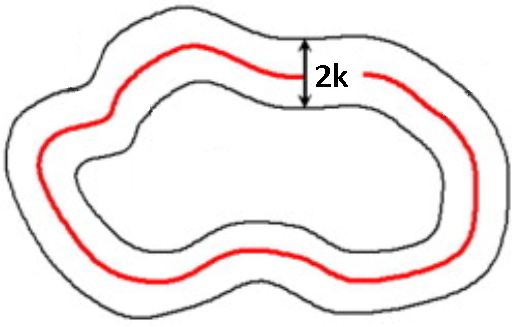
\includegraphics[width=.5\textwidth]{levelset/narrowBand}
\caption{The narrow band extending out with a width of k from the level set.}
\label{narrowBand}
\end{figure}
As the zero level set evolves, \(\phi\) will get further and further away from its initialized value as signed distance. As this happens \(\phi\) must be ensured to stay within the band. This can be accomplished by reinitializing \(\phi\) when the model gets close to the end of the band. The band have to be reset from the current position of the zero level set, and then \(\phi\) can be reinitialized. Reinitialize \(\phi\) at every iteration takes too much time and the alternative task of finding out if any of the pixels in the zero level set are getting close to the edge of the band (for every iteration) also takes time. Hence, \(\phi\) is usually just reinitialized after a fixed number of iterations, which keeps \(\phi\) approximately equal to the SDT. As metioned in the section about signed distance transforms, different SDTs can lead to slightly different end-results and must be carefully chosen. If the technique used to approximate \(\phi\) to a signed distance function is too sensitive, \(\phi\) needs to be reinitialized accurately and often. If it is less sensitive, it does not have to be initialized so often and a less accurate method can be used, but this may lead to noisy features \cite{osher02}.

The narrow band, despite its improvements over the original level set method, is not optimal. The band used being too wide is the main reason. Even if k=2 is enough to compute the necessary derivatives, the band have to be of a certain width (k=12 was used in the test of topological changes in \cite{adalsteinsson94}) because of two competing computional costs\cite{whitaker89}. The first is the cost of computing the position of the curve and the SDT, and reset the band. The second is the cost of computing the evolution process over the entire band.
